\section{Introduction}
\label{sec:intro}

% 3D reconstruction has rapidly progressed along two paradigms: optimization-based and feed-forward. Per-scene optimization methods \cite{mildenhall2021nerf,kerbl20233d,yu2024mip} can achieve high-fidelity reconstructions by iteratively minimizing photometric objectives on a single scene, but inference requires time-consuming scene-specific optimization, thus limiting practicality at scale. Moreover, while such pipelines benefit from per-iteration gradient error feedback, they typically do not inject external priors beyond network inductive biases and the given observed samples, leaving the potential of large datasets under-exploited.

Reconstructing 3D scenes from multi-view images is a fundamental task in computer vision, perception, and computer graphics, underpinning applications in robotic perception, AR/VR, and high-fidelity 3D content creation. 
3D reconstruction has rapidly progressed along two paradigms: per-scene optimization and feed-forward. Per-scene optimization methods \cite{mildenhall2021nerf,kerbl20233d,yu2024mip} can achieve high-fidelity reconstructions by iteratively minimizing photometric objectives on a single scene, but their inference requires long test-time gradient optimization, which limits scalability in real applications. In addition, while such pipelines benefit from iterative gradient feedback, they often struggle under sparse view inputs and do not effectively incorporate external data priors beyond inductive bias and observed samples, leaving the rich knowledge contained in large-scale 3D data underutilized.

\begin{figure}[t]
  \centering
  % 在双栏模板中，单栏宽度用 \columnwidth
  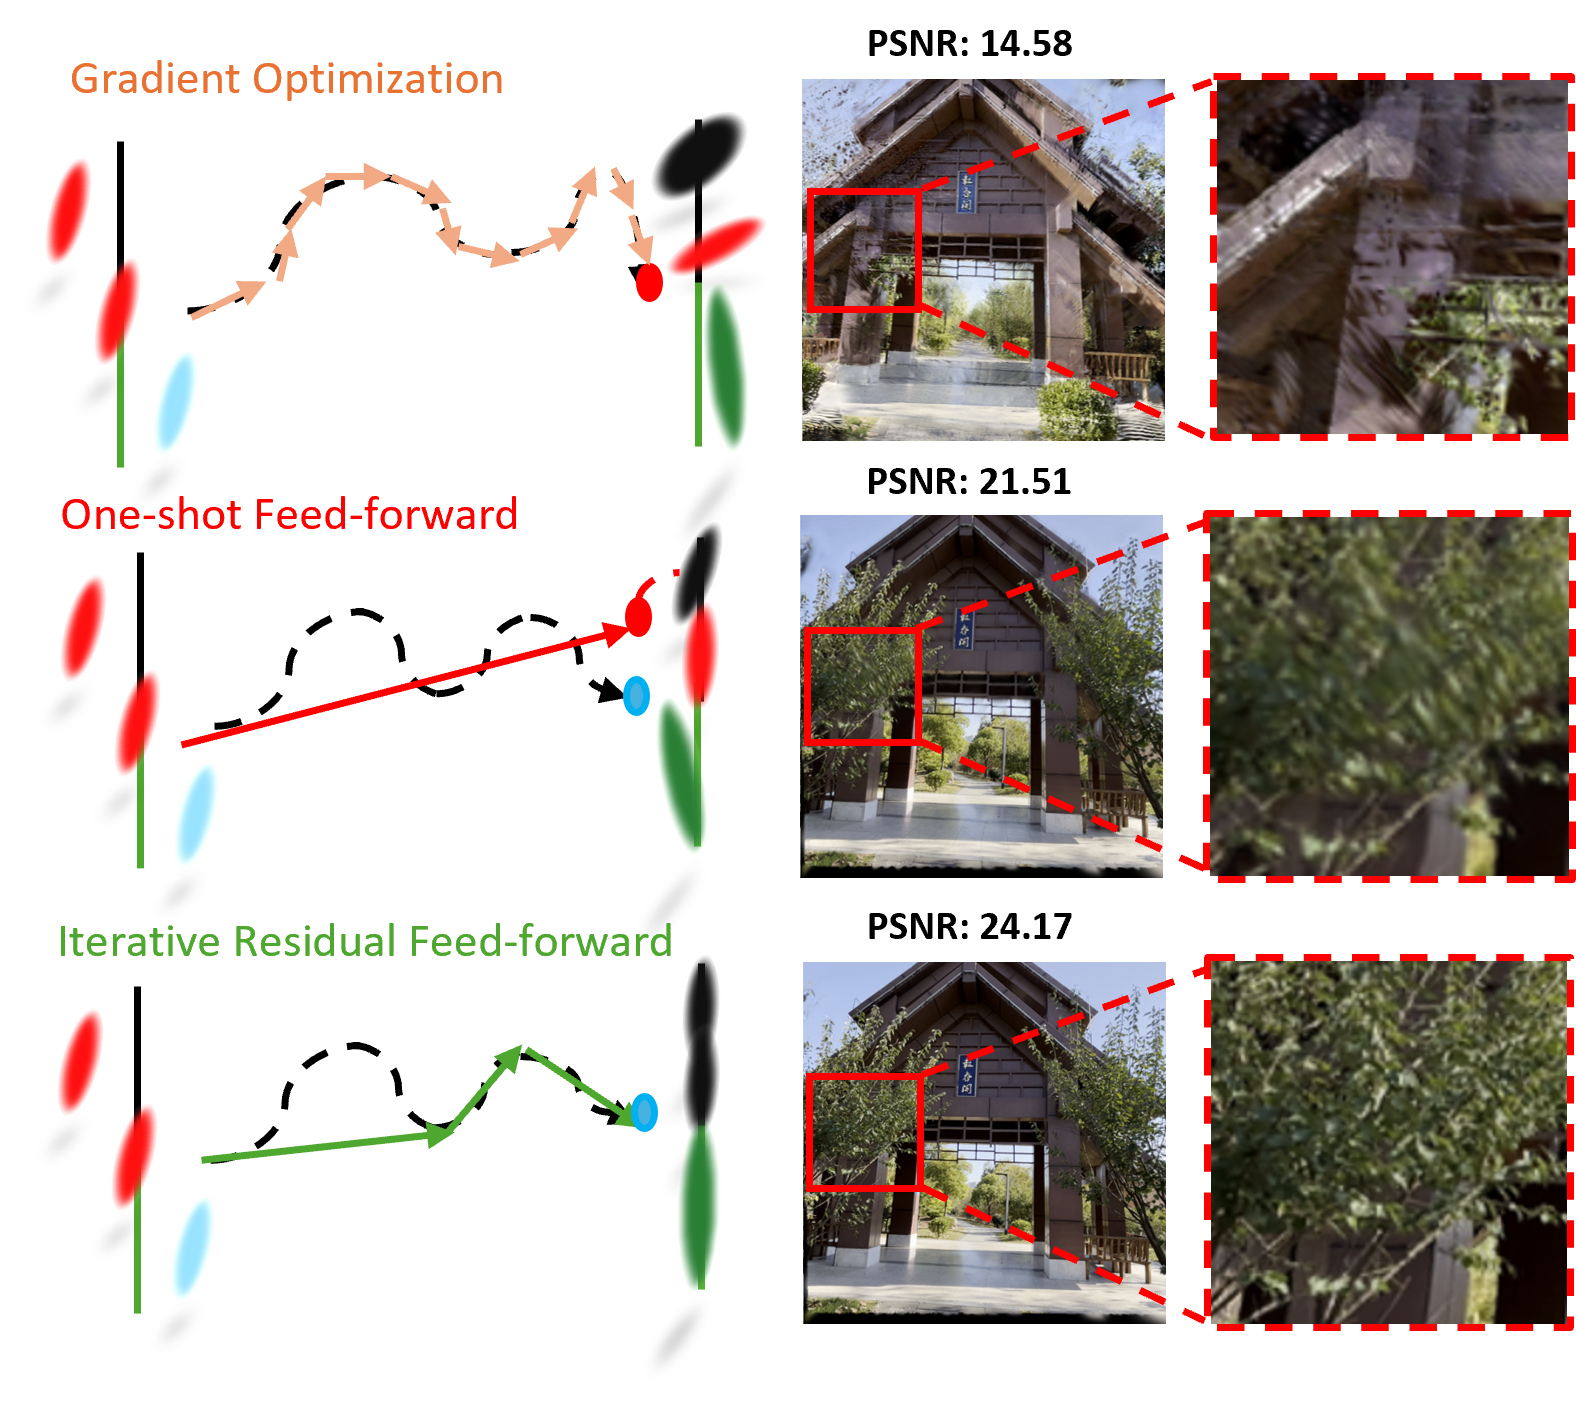
\includegraphics[width=0.95\columnwidth]{pics/intro.png}
  \caption{\textbf{Conceptual comparison of reconstruction paradigms.} Gradient optimization performs thousands updates, incurring heavy test-time cost, often achieving high quality in dense-view scenarios but struggling in sparse-view scenarios; One-shot feed-forward \cite{jiang2025anysplat} is efficient but leaves noticeable artifacts; Our iterative residual feed-forward scheme keeps feed-forward efficiency and achieves higher reconstruction quality without test-time gradient backpropagation.}
  \label{fig:1}
\end{figure}


% In contrast, recent feed-forward approaches \cite{wang2024dust3r, leroy2024grounding, yang2025fast3r, wang2025vggt} amortize multi-view reasoning into a single forward pass, delivering millisecond- to second-level runtimes and quality comparable to per-scene pipelines in some settings. However, most existing designs follow a one-shot prediction paradigm: a high-capacity backbone learns a direct mapping from input images to 3D attributes. This brings two fundamental limitations. First, performance is tightly constrained by model capacity; complex scenes expose the ceiling of a single-pass estimator. Second, generalization is bounded by the training data distribution; when facing out-of-domain sample, one-shot predictors often degrade noticeably as mentioned in some benchmark \cite{cong2025e3d}. Empirically, while large feed-forward model such as VGGT \cite{wang2025vggt} can infer plausible 3D attributes, additional bundle adjustment still yields substantial quality gains, indicating that a single pass leaves correctable residuals unmodeled.

% （Wu-old）In contrast, recent feed-forward approaches \cite{wang2024dust3r,leroy2024grounding,yang2025fast3r,wang2025vggt} (amortize multi-view reasoning into a single forward pass), achieving millisecond- to second-level runtime and delivering competitive quality in many settings. However, most existing methods follow a one-shot prediction paradigm, where a high-capacity model directly maps input images to 3D attributes without per-scene refinement. This paradigm faces three fundamental limitations. First, reconstruction quality is constrained by model capacity, and complex or cluttered scenes can expose the limits of a single-pass estimator. Second, one-shot prediction lacks a mechanism to refine geometry or appearance using scene-specific evidence, leaving correctable residuals unmodeled even in strong systems such as VGGT \cite{wang2025vggt}. Third, while generative priors could theoretically complement sparse or ambiguous observations, leveraging them reliably remains challenging in a purely feed-forward manner, as naive prior injection \cite{wu2025difix3d+} can introduce instability or require heavy test-time computation.

In contrast, recent feed-forward approaches ~\cite{wang2024dust3r,leroy2024grounding,yang2025fast3r,wang2025vggt} estimate 3D attributes from multi-view images in a single forward pass, incorporating multi-view interactions through an attention mechanism within Vision Transformers and employing dedicated attribute prediction heads, achieving millisecond- to second-scale inference time.
However, such one-shot prediction introduces two key limitations:
(1) its performance is constrained by model capacity, leading to lower fidelity in complex scenes; and
(2) it lacks scene-specific refinement, leaving residual errors uncorrected even in large-scale models \cite{wang2025vggt}.
%and (3) difficulty to keep efficient when incorporating generative priors \cite{wu2025difix3d+}.
Consequently, the core challenge remains: \emph{how to achieve feed-forward efficiency while enabling adaptation and continuous refinement to each scene.}% and efficient use of generative priors.

% These observations motivate an intermediate solution: retain feed-forward efficiency while enabling continuous refinement. The essence of feed-forward learning is to acquire dataset-level knowledge for the mapping from multi-view image to 3D; However, directly learning this mapping is intrinsically hard due to 3D data insufficiency and moreover the natural complexity of 3D structures compared to 2D assets. A promising remedy is to progressively refine under the knowledge from large-scale training: use fast forward predictions to obtain a strong initialization, then perform lightweight, learned residual updates driven by per-scene evidence.

% These observations motivate the need for an intermediate paradigm that preserves feed-forward efficiency while enabling reliable scene-specific refinement. While feed-forward models excel at capturing dataset-level priors for mapping sparse multi-view inputs to 3D structures, directly inferring a complete and accurate scene in a single pass remains intrinsically challenging due to the limited availability of high-quality 3D supervision and the inherent geometric and appearance complexity beyond 2D imagery. A promising direction is to combine amortized prediction with lightweight refinement: obtain a strong initialization through a fast forward pass, then apply learned residual updates guided by scene observations and prior knowledge, avoiding the cost and instability of test-time optimization.


However, generating artifact-free novel views remains challenging in complex scenes, particularly when view coverage is sparse \cite{kerbl20233d}. Recent studies \cite{wu2025difix3d+,wu2025genfusion} tend to address this limitation by integrating generative priors but require long-time per-scene optimization.
They alternatively optimize 3D Gaussians and refine rendered views with diffusion models, and these refined views are then fed back into the training set for further optimization, forming a feedback loop that gradually improves reconstruction quality. 
Yet this iterative loop is \emph{ill-suited} for existing feed-forward pipelines. As the continuously growing set of synthesized views increases both time and memory complexity, which are further exacerbated by the expensive self-attention operations in ViT-based backbones \cite{sharir2021image} adopted by recent feed-forward methods \cite{charatan2024pixelsplat, chen2024mvsplat, xu2025depthsplat, ye2024no, jiang2025anysplat}. Moreover, these methods reconstruct 3D scene directly from multi-view images rather than updating an existing scene representation, making iterative enhancement feedback infeasible, let alone step-wise fusion of generative priors. This raises an essential question: \emph{how to refine a 3D state in a purely feed-forward manner, leveraging both observations and generative priors while keeping second-scale inference runtime?}

% On the other hand, producing photorealistic novel view renderings remains challenging, despite impressive performance near inference viewpoints, existing 3D reconstruction methods \cite{kerbl20233d, mildenhall2021nerf} still suffer from artifacts, floaters, and texture sticking in novel views, especially under sparse view coverage, hampering their suitability to real-world settings. Recent methods \cite{wu2025difix3d+,wu2025genfusion,liu20243dgs} incorporate generative priors by alternating: (1) thousands of optimization steps to update 3D Gaussians; (2) diffusion-based enhancement of rendered novel views to remove artifacts; (3) feedback of the enhanced images into supervised image set; and (4) another round of optimize-based 3D Gaussians updates. While effective within optimization-based regimes, this loop is ill-suited for feed-forward pipelines: the ever-increasing synthesized views inflate time and space complexity, colliding with expensive self-attention mechanism of ViT \cite{sharir2021image} backbone in existing feed-forward methods \cite{charatan2024pixelsplat, chen2024mvsplat, xu2025depthsplat, ye2024no, jiang2025anysplat}; In addition, they reconstruct directly from multi-view images to 3D scene, rather than updating an existing scene state, making iterative use of enhancement feedback unplausible.

% On the other hand, producing artifact-free novel views remains challenging.
% Even state-of-the-art reconstruction pipelines \cite{kerbl20233d,mildenhall2021nerf} exhibit floaters, texture sticking, and view-dependent artifacts under sparse or wide-baseline inputs, limiting robustness in real-world usage.
% Recent work incorporates generative priors by alternating between 3D Gaussian optimization and diffusion-based image enhancement \cite{wu2025difix3d+,wu2025genfusion,liu20243dgs}, where enhanced novel views are repeatedly fed back into supervised training.
% While effective in optimization-based regimes, this strategy is poorly aligned with feed-forward pipelines: synthesized views accumulate over iterations, causing prohibitive time and memory growth, and the resulting large image batches clash with the expensive self-attention backbone used in modern one-shot models \cite{charatan2024pixelsplat,chen2024mvsplat,xu2025depthsplat,ye2024no,jiang2025anysplat}.
% Moreover, these approaches reconstruct scenes directly from input views rather than updating an existing 3D state, making iterative use of prior-enhanced cues infeasible without reverting to costly test-time optimization.
To tackle this challenge, we propose GIFSplat, an iterative feed-forward 3D Gaussian Splatting framework that leverages the strengths of both feed-forward and optimization-based methods. The first stage performs a fast feed-forward pass to produce a reliable initialization, and the second stage refines an initial prediction through multi-step forward-only residual updates guided by scene evidence and diffusion-enhanced cues. 
GIFSplat maintains the speed of feed-forward pipeline while enabling scene-adaptive refinement and reliable prior injection, bridging the gap between one-shot feed-forward methods and optimization-based pipelines.
At each step, GIFSplat uses the current Gaussian state and discrepancy cues to predict residual updates.
This allows continuous improvement without test-time gradient backpropagation, with memory and runtime scaling linearly in the number of refinement steps. A conceptual comparison of paradigms is shown in ~\cref{fig:1}.
Rather than continuously extending supervised image sets with enhancing rendered images then re-optimizing the scene, we apply a diffusion enhancer \cite{wu2025difix3d+} to novel rendered images, extract enhancement deltas, and convert them into prior guidance cue. This approach brings reliable priors without view explosion and followed heavy computation.


% In the paper, we alleviate above problem by propose \textit{GIFSplat}, an iterative feed-forward 3DGS prediction framework with generative prior, which followed by two design : 
% (1) From model aspect (Section\ref{sec:iter_Gaussian_head} iterative residual refinement), instead of time-consuming gradient back-propagating at test time, GIFSplat performs fast multi-step forward residual updates; an iterative residual Gaussians module conditions on the current 3D Gaussians, features and error signals derived from rendered views and their generative-prior-enhanced counterparts, then predicts residuals to Gaussians. By continuously feedback rendered error to the iterative Gaussian head, GIFSplat avoids view explosion, keeps memory/time linear in the number of lightweight updates, and realizes continuous refinement within a feed-forward paradigm. 
% (2) From the data aspect (Section\ref{sec:prior_fusion} fusion of generative prior), the generative prior is used not to re-optimize the whole scene but to denoise and amplify information from enhanced novel-view renderings; these distilled signals guide subsequent residual predictions without invoking thousands of optimization steps. We compared our method with other paradigms in Figure 1.

% To address the above challenges, we introduce GIFSplat, an iterative feed-forward 3D Gaussian Splatting framework that leverages generative priors while maintaining feed-forward efficiency.
% GIFSplat is built upon two key design principles:
% (1) Iterative residual refinement (Section~\ref{sec:iter_Gaussian_head}).
% Instead of time-consuming gradient-based test-time optimization, GIFSplat performs fast multi-step forward-only residual updates.
% At each iteration, the residual Gaussian module conditions on the current Gaussian state, corresponding features, and error cues from both rendered views and their generative-prior-enhanced counterparts, and predicts updates to Gaussian parameters.
% By continuously feeding rendered discrepancies back into the refinement loop, GIFSplat avoids view explosion, keeps memory and runtime linear in the number of refinement steps, and enables test-time scene adaptation within a purely feed-forward paradigm.
% (2) Conservative generative-prior fusion (Section~\ref{sec:prior_fusion}).
% Rather than re-optimizing the entire scene, GIFSplat uses the generative prior to denoise and amplify cues in novel-view renderings, distilling them into lightweight guidance signals that steer subsequent residual updates.
% This enables prior-aware refinement without thousands of optimization steps or unstable direct prior injection.
% A comparison with existing paradigms is provided in Figure~\ref{fig:1}.


% Specifically, GIFSplat alternates the residual-update in a forward-only loop: render from multiple viewpoints including input and novel views; apply a diffusion-based enhancer \cite{wu2025difix3d+} to suppress artifacts and hallucinate plausible details in novel views as pesudo-supervision; compute discrepancy cues between rendered and correspondent supervised images; and fuse these cues with current multi-view evidence to predict compact residuals on 3D Gaussians. This design preserves the speed of feed-forward inference while injecting prior-aware corrections, yielding reconstructions that are sharper and more complete, particularly under the scenario of domain shift or sparse coverage. 

% Specifically, GIFSplat performs residual refinement in a forward-only loop.
% At each step, we render both input and novel viewpoints, enhance the rendered novel views with a diffusion-based prior \cite{wu2025difix3d+} to suppress artifacts and hallucinate plausible high-frequency details, and then compute discrepancy cues between rendered images and their enhanced counterparts.
% These cues, combined with current multi-view observations, are fused to predict compact residual updates on the 3D Gaussians.
% By iteratively applying such lightweight forward updates, GIFSplat maintains feed-forward efficiency while introducing reliable prior-aware corrections, enabling sharper and more complete reconstructions, especially under sparse views or domain shift.

% Our contribution can be summarized as follows:

% \noindent (1) We propose GIFSplat, an iterative feed-forward 3DGS prediction framework with generative priro that performs multi-step forward residual updates to achieve efficient scene-level refinement without thousands of steps of explicit optimization of gradient descent.

% \noindent (2) We design a prior-aware update mechanism that distills generative priors from enhanced novel-view renderings into error signals, directly driving update to 3D Gaussians in each step while avoiding the memory explosion caused by self-attention of increasing views.

% \noindent (3) Across diverse dataset (DL3DV, RealEstate10K, DTU) and settings (different overlap ratio), our IFSplat and GIFSplat with generative prior delivers consistent improvements over strong feed-forward baselines.

% Our contributions are threefold: (1) We introduce GIFSplat, an iterative feed-forward 3D Gaussian Splatting with generative prior framework that performs multi-step forward-only residual refinement, enabling efficient scene-specific adaptation without test-time gradient descent. (2) We propose a prior-aware refinement mechanism that distills generative priors from enhanced novel-views into discrepancy prior cues, guiding Gaussian updates in iterative steps without increasing reference views. (3) We demonstrate consistent performance gains across DL3DV, RealEstate10K, and DTU dataset, under varying view-overlap settings, showing that our iterative feed-forward model (IFSplat) and generative-prior variant (GIFSplat) both outperform recent feed-forward reconstruction methods in sparse-view and cross-domain scenarios.
%\noindent

The primary contributions of this work are as follows:
\begin{itemize}
\item We present an iterative feed-forward update mechanism for 3D Gaussian Splatting that refines a fixed set of Gaussians via multi-step, forward-only residual updates, enabling scene-specific refinement without any test-time gradient descent.

\item We introduce a generative prior fusion mechanism that distills a frozen diffusion prior into lightweight Gaussian-level discrepancy cues from enhanced novel renderings, injecting generative information into the iterative updates without backpropagation or continuously expanding the set of reference views.

\item We demonstrate consistent performance gains across DL3DV, RealEstate10K, and DTU datasets, under varying view-overlap settings, showing that our iterative feed-forward model (IFSplat) and generative-prior variant (GIFSplat) both outperform recent feed-forward reconstruction methods in sparse-view and cross-domain scenarios.
\end{itemize}
%Across diverse data settings, especially out-of-domain scenes, GIFSplat delivers consistent improvements over strong feed-forward baselines.

% \begin{figure}[t]
%   \centering
%   % 在双栏模板中，单栏宽度用 \columnwidth
%   \placeholderbox[0.95\columnwidth]{45mm}
%   \caption{Diagram of three paradigm. Optimization-based method only rely on gradient to update; One-shot Feed-forward directly predict result from input multi-view images with learned knowledge; Iterative Feed-forward Refinement progressively update current 3D Gaussians under with learned knowledge.}
%   \label{fig:single}
% \end{figure}



% \begin{figure}[t]
%   \centering
%   % 在双栏模板中，单栏宽度用 \columnwidth
%   \includegraphics[width=.95\linewidth]{pics/underconstrain.png}
%   \caption{Low quality rendered image in under-constrained viewpoint}
%   \label{fig:single}
% \end{figure}


